\documentclass[10pt,letterpaper]{article}
\usepackage[margin=0.68in,headheight=14pt,headsep=12pt,footskip=24pt]{geometry}
\usepackage[T1]{fontenc}
\usepackage{lmodern,amsmath,booktabs,tabularx,xcolor,fancyhdr}
\usepackage{pgfplots}
\usepackage[colorlinks=true,urlcolor=teal!65!black,linkcolor=teal!65!black,citecolor=teal!65!black]{hyperref}
\pgfplotsset{compat=1.18}
\definecolor{ink}{HTML}{183244}
\definecolor{accent}{HTML}{087F8C}
\definecolor{pale}{HTML}{EFF6F7}
\setlength{\parindent}{0pt}
\setlength{\parskip}{4pt}
\setlength{\tabcolsep}{4pt}
\renewcommand{\arraystretch}{1.10}
\pagestyle{fancy}\fancyhf{}
\fancyhead[L]{\small\sffamily\color{ink}CancerOmicsLake}
\fancyhead[R]{\small\sffamily Research synopsis v2 \textbar\ 19 October 2026}
\fancyfoot[L]{\small Pronab Chandra Roy}
\fancyfoot[R]{\small\thepage\ / 4}
\renewcommand{\headrulewidth}{0.3pt}
\newcommand{\topic}[1]{\par\vspace{4pt}{\large\sffamily\bfseries\color{ink}#1}\par\vspace{1pt}}
\newcommand{\subtopic}[1]{\par\vspace{2pt}{\bfseries\color{ink}#1}\par}
\newcommand{\takeaway}[1]{\par\smallskip\noindent\colorbox{pale}{\parbox{\dimexpr\linewidth-2\fboxsep\relax}{\textbf{Interpretation.} #1}}\par}
\tikzset{stage/.style={draw=accent,fill=pale,rounded corners=2pt,align=center,text width=4.1cm,minimum height=0.76cm,font=\footnotesize},route/.style={->,draw=accent,thick},labelbox/.style={align=center,font=\footnotesize,text width=5.1cm}}
% Generated from checked aggregate evidence.
\newcommand{\TCGARows}{36,456,660}
\newcommand{\GTExRows}{11,240,000}
\newcommand{\NativeScripts}{7}
\newcommand{\WorkflowCells}{21}
\newcommand{\MatchedTCGA}{417}
\newcommand{\PrimaryNormals}{150}
\newcommand{\PrimarySpecimens}{567}
\newcommand{\SharedGenes}{55,660}
\newcommand{\MatchedTotal}{617}
\newcommand{\MatchedGTEx}{200}
\newcommand{\SigmoidNormals}{50}
\newcommand{\MatchedRows}{BRCA & 162 & 50 & 0.559 & 89.85\% & 23,247 & 0.0046 \\
COAD & 119 & 50 & 0.556 & 90.53\% & 22,007 & 0.0026 \\
LUAD & 136 & 50 & 0.571 & 90.21\% & 23,732 & 0.0058 \\}
\newcommand{\CohortRows}{BRCA & 162 & 50 & 89.85\% & 23,247 \\
COAD & 119 & 50 & 90.53\% & 22,007 \\
LUAD & 136 & 50 & 90.21\% & 23,732 \\}
\newcommand{\TieMin}{412}
\newcommand{\TieMax}{515}
\newcommand{\NativeFailed}{63}
\newcommand{\NativeSensitivityTotal}{8,100}
\newcommand{\PairedFailed}{60}
\newcommand{\PairedSensitivityTotal}{8,100}
\newcommand{\RankingDesignCounts}{BRCA 26/24, COAD 21/20, LUAD 26/24}
\newcommand{\ExactComparisons}{46}
\newcommand{\ExactAttempts}{6,624}
\newcommand{\ExactFailed}{36}
\newcommand{\ContractCases}{32}
\newcommand{\ContractDecisions}{192}
\newcommand{\RecomputeEvents}{400}
\newcommand{\RecomputeWorkloads}{40}
\newcommand{\CertifiedEvents}{233}
\newcommand{\LifecycleWins}{0}
\newcommand{\AbstentionDatasets}{3,600}
\newcommand{\JointWrong}{47}
\newcommand{\HolmWrong}{5}
\newcommand{\FragilityWorlds}{112}
\newcommand{\FragilityCases}{7}
\newcommand{\TieDraws}{1,000}
\newcommand{\BioBootstraps}{200}
\newcommand{\BootstrapTieDraws}{100}
\newcommand{\DirectionThreshold}{0.2}
\newcommand{\DetectionPercent}{20}

\hypersetup{pdftitle={CancerOmicsLake: reproducibility and the sensitivity of candidate-gene rankings},pdfauthor={Pronab Chandra Roy}}
\begin{document}
{\sffamily\color{accent}\small BIOINFORMATICS DATA ENGINEERING \ / \ PHD RESEARCH SYNOPSIS}\par
{\sffamily\bfseries\color{ink}\LARGE CancerOmicsLake}\par
{\sffamily\color{ink}\Large Reproducibility and the sensitivity of\newline candidate-gene rankings}\par
\textbf{Pronab Chandra Roy}\hfill\href{https://github.com/pronabroy360/CancerOmicsLake}{Project repository and source code}\par

\topic{1. Question and contribution}
\textbf{Does agreement across a broad gene-expression profile justify confidence
in its leading candidate genes?} We built CancerOmicsLake to measure how
reference choice, processing, ties and numerical execution affect that inference.
The main empirical result is that moderate signed-effect concordance coexists
with very weak top-50 overlap in exactly matched native/recount3 comparisons.
The contribution combines an implemented data platform with an auditable
sensitivity evaluation; processing variability itself is established prior
work~\cite{arora,recount}.

\subtopic{System and data}
The platform integrates open-access GDC/TCGA expression, mutation and metadata
with GTEx normals, gene annotations and public recount3 processed expression.
It covers breast invasive carcinoma (BRCA), lung adenocarcinoma (LUAD) and colon
adenocarcinoma (COAD), with breast, lung and two colon reference tissues.
The frozen expression inventory contains \textbf{\TCGARows\ TCGA} and
\textbf{\GTExRows\ GTEx} measurement rows. These are gene--specimen values,
not counts of patients or sequencing files.

\begin{center}
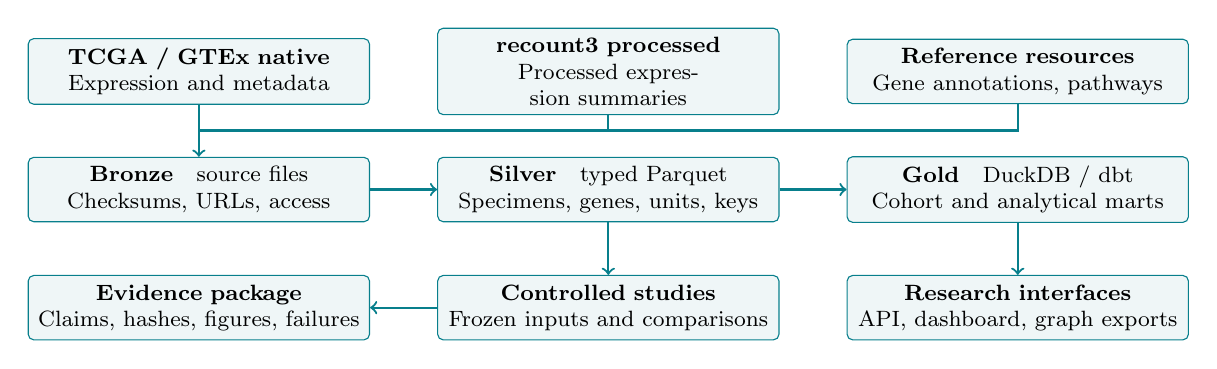
\begin{tikzpicture}
\node[stage] (tcga) at (0,0) {\textbf{TCGA / GTEx native}\\Expression and metadata};
\node[stage] (recount) at (5.2,0) {\textbf{recount3 processed}\\Processed expression summaries};
\node[stage] (ref) at (10.4,0) {\textbf{Reference resources}\\Gene annotations, pathways};
\node[stage] (bronze) at (0,-1.5) {\textbf{Bronze}\quad source files\\Checksums, URLs, access};
\node[stage] (silver) at (5.2,-1.5) {\textbf{Silver}\quad typed Parquet\\Specimens, genes, units, keys};
\node[stage] (gold) at (10.4,-1.5) {\textbf{Gold}\quad DuckDB / dbt\\Cohort and analytical marts};
\draw[accent,thick] (tcga.south) -- (0,-0.75) -- (10.4,-0.75) -- (ref.south);
\draw[accent,thick] (recount.south) -- (5.2,-0.75);
\draw[route] (0,-0.75) -- (bronze.north);
\draw[route] (bronze) -- (silver);
\draw[route] (silver) -- (gold);
\node[stage] (evidence) at (0,-3.0) {\textbf{Evidence package}\\Claims, hashes, figures, failures};
\node[stage] (studies) at (5.2,-3.0) {\textbf{Controlled studies}\\Frozen inputs and comparisons};
\node[stage] (serve) at (10.4,-3.0) {\textbf{Research interfaces}\\API, dashboard, graph exports};
\draw[route] (silver) -- (studies);
\draw[route] (studies) -- (evidence);
\draw[route] (gold) -- (serve);
\end{tikzpicture}
\end{center}
{\footnotesize\textbf{Figure 1. Implemented workflow.} Acquisition preserves
source context; harmonization validates entities and measurements before
analytical use. Frozen study inputs connect analytical outputs to claim-level
evidence. Arrows denote data dependencies, not validation of biological truth.}\par

\subtopic{What was implemented and evaluated}
Python/Polars transformations, DuckDB/dbt models, orchestration, Docker and CI
support configured ingestion, bounded downloads, retries and validation.
Streamlit, FastAPI and Neo4j/Graphify exports expose the analytical layers.
Exploratory analytics include consequence-stratified mutation frequencies,
expression comparisons, candidate rankings, pathway overrepresentation with
within-cancer/candidate-set BH correction, and graph degree summaries.

The evaluated contribution has three parts: (i) specimen/gene harmonization and
source-to-claim traceability; (ii) matched processing and reference-sensitivity
studies with uncertainty diagnostics; and (iii) numerical replay and external
baseline/failure tests. Repairs addressed duplicate keys, preservation of
\texttt{\_PAR\_Y} loci and donor/case leakage. Earlier evidence is retained when
later designs change. Mutation, pathway and graph summaries provide context;
they are not independent biological validation of the rankings.

\takeaway{The platform makes the conditions behind a candidate list inspectable.
The research evaluates its reliability and limitations rather than treating a
successful execution as evidence of a stable scientific conclusion.}

\newpage
\topic{2. Matched processing study: design and principal result}
Exact identity, case/donor, tissue, QC and count-column checks yielded
\textbf{\MatchedTotal\ available specimens}: \MatchedTCGA\ tumors and
\MatchedGTEx\ GTEx normals. The three primary contrasts use
\textbf{\PrimarySpecimens\ specimens} (\MatchedTCGA\ tumors plus
\PrimaryNormals\ normals); \SigmoidNormals\ sigmoid-colon normals are retained
separately. COAD's primary reference is transverse colon. V2 followed inspection
of v1 and is an exploratory diagnostic study.

\begin{center}
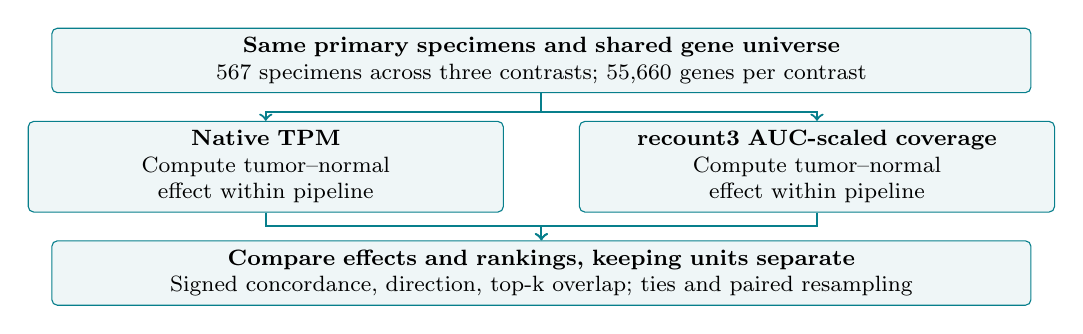
\begin{tikzpicture}
\node[stage,text width=12.2cm] (match) at (3.5,0) {\textbf{Same primary specimens and shared gene universe}\\\PrimarySpecimens\ specimens across three contrasts; \SharedGenes\ genes per contrast};
\node[stage,text width=5.8cm] (native) at (0,-1.35) {\textbf{Native TPM}\\Compute tumor--normal effect within pipeline};
\node[stage,text width=5.8cm] (uniform) at (7,-1.35) {\textbf{recount3 AUC-scaled coverage}\\Compute tumor--normal effect within pipeline};
\node[stage,text width=12.2cm] (compare) at (3.5,-2.7) {\textbf{Compare effects and rankings, keeping units separate}\\Signed concordance, direction, top-k overlap; ties and paired resampling};
\draw[route] (match.south) -- (3.5,-0.65) -| (native.north);
\draw[route] (3.5,-0.65) -| (uniform.north);
\draw[route] (native.south) -- (0,-2.1) -| (compare.north);
\draw[route] (uniform.south) -- (7,-2.1) -| (compare.north);
\end{tikzpicture}
\end{center}
{\footnotesize\textbf{Figure 2. Matched comparison.} Membership is fixed across
pipelines. Each gene's rank-biserial effect is the empirical probability that a
tumor value exceeds a normal value minus the reverse probability, ranging from
$-1$ to $1$. This rank-based contrast does not make numerical units equivalent.}\par

\begin{center}\small
\begin{tabular}{lrrcr}
\toprule
Cancer & Tumors & GTEx normals & Direction agreement & Eligible genes\\
\midrule
\CohortRows
\bottomrule
\end{tabular}\end{center}
{\footnotesize Direction agreement is conditional on $|r_g|\geq\DirectionThreshold$
in both pipelines. Its gene denominator is shown; it is not a proportion of specimens.}\par

\begin{center}
\begin{tikzpicture}
\begin{axis}[width=0.46\linewidth,height=1.45in,xmin=0.50,xmax=0.65,
 xtick={0.50,0.55,0.60,0.65},symbolic y coords={LUAD,COAD,BRCA},ytick=data,
 title={\small Signed-effect concordance},xlabel={\small Kendall $\tau_b$},
 tick label style={font=\footnotesize},axis lines*=left,xmajorgrids,grid style={gray!15}]
\addplot+[only marks,mark=*,color=accent,mark options={fill=accent,draw=accent},error bars/.cd,x dir=both,x explicit]
 table[y=cancer,x=tau,x error minus=tauMinus,x error plus=tauPlus]{matched_metrics.dat};
\end{axis}
\end{tikzpicture}\hfill
\begin{tikzpicture}
\begin{axis}[width=0.46\linewidth,height=1.45in,xmin=0,xmax=0.02,
 xtick={0,0.01,0.02},scaled x ticks=false,
 xticklabel style={/pgf/number format/fixed,/pgf/number format/precision=2},
 symbolic y coords={LUAD,COAD,BRCA},ytick=data,
 title={\small Leading-list overlap},xlabel={\small Tie-averaged top-50 Jaccard},
 tick label style={font=\footnotesize},axis lines*=left,xmajorgrids,grid style={gray!15}]
\addplot+[only marks,mark=*,color=ink,mark options={fill=ink,draw=ink},error bars/.cd,x dir=both,x explicit]
 table[y=cancer,x=jaccard,x error minus=jMinus,x error plus=jPlus]{matched_metrics.dat};
\end{axis}
\end{tikzpicture}
\end{center}
{\footnotesize\textbf{Figure 3. Broad agreement coexists with weak leading lists.}
Points show observed $\tau_b$ or mean tie-resolved Jaccard; bars show descriptive
95\% paired case/donor bootstrap percentile intervals (\BioBootstraps\ replicates).
Top-50 lists rank absolute effects. Axes use different ranges and statistics;
magnitudes are not directly comparable.}\par

Across all shared genes, $\tau_b$ was 0.556--0.571 while mean top-50 Jaccard was
0.0026--0.0058. Native cutoff ties spanned \TieMin--\TieMax\ genes. V2 separately
reported tie-only variability (\TieDraws\ seeded resolutions) and bootstrap
intervals with \BootstrapTieDraws\ tie resolutions per replicate. A fixed
\DetectionPercent\% detection filter in both groups/pipelines improved broad
concordance but did not rescue short lists. These descriptive results are
conditional on available matched specimens; processing and annotation causes
were not experimentally separated.

\newpage
\topic{3. Reference and reproducibility studies}
\subtopic{Does a more elaborate score beat a simple reference baseline?}
Separate corrected native and paired reference studies compared adjacent-normal
and GTEx controls with globally separated case/donor partitions. Within each
partition, tumor specimens and reference sizes were matched across methods.
Selected development/holdout counts \emph{per group} were \RankingDesignCounts\
in each design. These smaller ranking cohorts differ from the processing study
on p.~2; paired designs additionally constrain tumor/adjacent-normal case matching.

A bootstrap lower-quantile score was compared with single-reference effects,
mean ranks, maximin and the official R \texttt{RobustRankAggreg} implementation~\cite{rra}.
Top-25/50/100 evaluation used heldout effect/direction summaries and paired
resampling; reference ablations and bootstrap rank stability were exploratory
diagnostics. The proposed score had \textbf{no top-50 advantage over maximin}.
RRA was evaluated as a ranking: shared tumor specimens invalidate an
independent-list significance interpretation. Constructed shared-normal bias
also produced reference agreement with incorrect biological selections.

\subtopic{What reproduced, and what failed the original numerical gate?}
Archived replay compared macOS/Linux with pinned dependencies and Polars
1.42.1/1.44.2, retaining $\mathrm{rtol}=10^{-8}$ and
$\mathrm{atol}=10^{-10}$. Ordering, ties and intermediate arrays were recorded.
Three historical failed rows repeated one Spearman statistic at three top-k
values. The earliest observed divergence was in log2 effect arrays; the
underlying platform cause was not established by varying dependencies.

Candidate lists and heldout metrics reproduced in the corrected global studies.
However, \textbf{\NativeFailed/\NativeSensitivityTotal\ native and
\PairedFailed/\PairedSensitivityTotal\ paired values} of the
\texttt{abs\_effect\_spearman} sensitivity column exceeded tolerance. These are
failed scalar comparisons, not failed specimens or entire candidate lists.
Existing eager rational, specialized rational and CGAL lazy exact methods later
agreed in all \ExactComparisons\ workload/specification comparisons, including
native macOS checks. Of \ExactAttempts\ process attempts, \ExactFailed\ binary64
attempts failed on a constructed extreme-value fixture. This later study did
not repair the historical floating-point acceptance failures.

\subtopic{External preparation comparison and failure recovery}
The pinned \texttt{tcga-data-nf} implementation~\cite{workflow} was compared on
cached recount3 data with matching membership and normalization/filter semantics.
Outputs matched in \WorkflowCells\ preparation workloads and \NativeScripts\
native-script integrations. Equivalence preceded timing. The shared R
normalization backend, added adapter and emulated hardware restrict performance
interpretation; end-to-end Nextflow and intrinsic engine-speed superiority were
not established.

\begin{center}\small
\begin{tabularx}{\linewidth}{@{}>{\raggedright\arraybackslash}p{0.23\linewidth}>{\raggedright\arraybackslash}X>{\raggedright\arraybackslash}X@{}}
\toprule
Test & Observed result & What it establishes\\
\midrule
Corrupt input, missing metadata, conflicting duplicates & Benchmark adapter/parser rejected each & Detection at the recorded validation layer.\\
Interrupted execution & No incorrect output committed; fresh retry recovered & Recovery with an explicit pause hook, not native automatic resume.\\
Stale cached evidence & Evidence hash guard rejected reuse & Local evidence integrity; external native handling unmeasured.\\
Frozen sources and reports & Inputs, plans and earlier failures retained & An audit trail, not authentication of original biological assertions.\\
\bottomrule
\end{tabularx}\end{center}

\takeaway{The evidence supports controlled comparison and traceability. It also
records numerical failures and the absence of ranking/performance superiority;
passing software tests does not cancel these scientific limitations.}

\newpage
\topic{4. Method experiments and research scope}
Additional exploratory studies tested whether the observed failure modes
motivated a distinct method or systems benefit. Each addressed a bounded
question and used declared comparators. None established a superior new method.

\begin{center}\small
\begin{tabularx}{\linewidth}{@{}>{\raggedright\arraybackslash}p{0.23\linewidth}>{\raggedright\arraybackslash}X>{\raggedright\arraybackslash}X@{}}
\toprule
Study & Executed evidence & Result and interpretation\\
\midrule
Evidence contracts & \ContractCases\ synthetic cases; \ContractDecisions\ tool/case/pass decisions & SQL, SHACL and workflow gating matched the prototype. All admitted two false attestations.\\
Decision-aware recomputation & \RecomputeEvents\ distinct patch events in \RecomputeWorkloads\ workloads; \CertifiedEvents\ unchanged sets certified & No decision mismatches; lifecycle cost beat exact incremental updating in \LifecycleWins/\RecomputeWorkloads\ workloads.\\
Exact ranking arithmetic & \ExactComparisons\ comparisons of established exact methods & Agreement demonstrated; no unique capability or uniformly fastest implementation.\\
Selection with abstention & \AbstentionDatasets\ synthetic datasets; Holm, Bonferroni and joint bootstrap & The narrow top-k label gate passed, but invalid pair directions occurred in \JointWrong/200 versus \HolmWrong/200 datasets in one moderate-signal cell.\\
Minimum claim-flipping changes & \FragilityWorlds\ synthetic alternatives in \FragilityCases\ scenarios & SQL and Python agreed on all decisions and minimum-change witnesses. Actual quantification-workflow generation was untested.\\
\bottomrule
\end{tabularx}\end{center}
{\footnotesize Repeated timings/tool passes are not independent datasets.
The abstention example uses 30 donors. Its pairwise error prevents a calibrated
confidence claim despite correct observed top-k labels. The official confident
feature-ranking implementation~\cite{confident} was not benchmarked.}\par

\subtopic{Relationship to the literature}
Arora et al.~\cite{arora} already established that pipeline choice affects
expression and downstream results. Recount3~\cite{recount} supplies uniformly
processed expression; RRA~\cite{rra} and confident feature ranks~\cite{confident}
provide established ranking methods. CancerOmicsLake's contribution is an
implemented, auditable case study linking matched effect rankings, tie
uncertainty, numerical replay and failure-aware evidence packaging.

Arora replication remains unexecuted: checked expression-archive locations
returned access errors on 16 October 2026. This does not show that the matrices
were never published. Their endpoints and ours are not a matched head-to-head
benchmark. The external preparation comparison has the scope stated on p.~3.

\subtopic{Scope of inference and remaining work}
The project demonstrates biomedical data engineering and a substantive
sensitivity evaluation. Its strongest finding is the distinction between broad
effect agreement, short-list stability and numerical acceptance. Annotation,
processing, collection and batch effects were not causally separated. Only
three cancers and available matched specimens were examined; inspected holdouts
are development evidence. Neither clinical utility nor biological validation
has been demonstrated.

The next requirements are independent investigator reproduction of the prepared
handoff, external evaluation on identical endpoints and fresh evidence selected
before further method tuning. A future algorithm would need an explicit
estimand and improvement over competent baselines, including maximin. This
platform is an implemented starting point for my PhD interest in reliable
biomedical data infrastructure and reproducible analysis.

{\footnotesize\textbf{Status.} Four-page research synopsis for interview
 discussion; detailed methods and evidence accompany the repository. AI tools
 assisted implementation and drafting. Author review and formal declarations
 remain to be finalized; independent human reproduction is pending.}\par

\vspace{-3pt}
\begin{thebibliography}{5}\footnotesize\raggedright\setlength{\itemsep}{0pt}\setlength{\parskip}{0pt}
\bibitem{arora} Arora et al. \emph{Variability in estimated gene expression among commonly used RNA-seq pipelines}. Scientific Reports, 2020. \href{https://doi.org/10.1038/s41598-020-59516-z}{doi:10.1038/s41598-020-59516-z}.
\bibitem{recount} Wilks et al. \emph{recount3: summaries and queries for large-scale RNA-seq expression and splicing}. Genome Biology, 2021. \href{https://doi.org/10.1186/s13059-021-02533-6}{doi:10.1186/s13059-021-02533-6}.
\bibitem{rra} Kolde et al. \emph{Robust rank aggregation for gene list integration and meta-analysis}. Bioinformatics, 2012. \href{https://doi.org/10.1093/bioinformatics/btr709}{doi:10.1093/bioinformatics/btr709}.
\bibitem{workflow} Quackenbush Lab. \emph{tcga-data-nf}. \href{https://github.com/QuackenbushLab/tcga-data-nf/tree/1069eb9c01b97640fd532ffac8551096d2a2790a}{Pinned workflow source}; limited comparison on p.~3.
\bibitem{confident} Neuhof and Benjamini. \emph{Confident Feature Ranking}. AISTATS, 2024. \href{https://proceedings.mlr.press/v238/neuhof24a.html}{PMLR 238:1468--1476}.
\end{thebibliography}
\end{document}
